\documentclass{article}
\usepackage[utf8]{inputenc}

\usepackage{tikz}
\usepackage[siunitx]{circuitikz}
\usetikzlibrary{circuits.logic.US}
\usetikzlibrary{positioning}
\usetikzlibrary{shapes}
\usetikzlibrary{calc}
\begin{document}
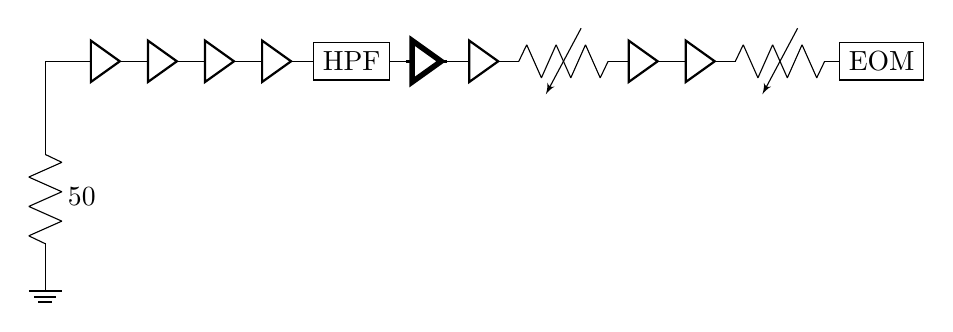
\begin{tikzpicture}[circuit logic US, >=latex]

\ctikzset{bipoles/buffer/height=.375} 
\ctikzset{bipoles/buffer/width=.375} 
\ctikzset{bipoles/thickness=1}
%\ctikzset{bipoles/buffer/thickness=1}

\node[draw] (eom) at (0,0) {EOM};

\def \ampsep{.2}

\draw (eom.west) to[vR] ++(-1.5, 0) node[buffer, anchor=out] (amp2) {}
    (amp2.in) to[short] ++ (-\ampsep, 0) node[buffer, anchor=out] (amp1) {}
    (amp1.in) to[vR] ++(-1.5, 0) node[buffer, anchor=out] (preamp6) {}
    (preamp6.in) to[short] ++ (-\ampsep, 0) node[buffer, anchor=out, line width=1] (preamp5) {}
    (preamp5.in) to[short] ++ (-\ampsep, 0) node[draw, anchor=east] (hpf) {HPF}
    (hpf.west) to[short] ++(-\ampsep, 0) node[buffer, anchor=out] (preamp4) {}
    (preamp4.in) to[short] ++(-\ampsep, 0) node[buffer, anchor=out] (preamp3) {}
    (preamp3.in) to[short] ++(-\ampsep, 0) node[buffer, anchor=out] (preamp2) {}
    (preamp2.in) to[short] ++(-\ampsep, 0) node[buffer, anchor=out] (preamp1) {}
    (preamp1.in) -| ++(-.5, -1) to[R=50] ++(0, -1.5)  node[ground] {}
    ;


\end{tikzpicture}
\end{document}